\lesson{3}{25.09.2023}{Матрицы}
\section{Матрицы}

\begin{definition}
    Пусть V --- конечное мерное пространство

    $v_1 \ldots v_n$ - базис V

    $w \in V \implies \exists! \alpha_1, \alpha_2, \ldots, \alpha_n:$

    $w = \alpha_1 \cdot v_1 + \alpha_2 \cdot v_2 + \ldots + \alpha_n \cdot v_n$

    Тогда $\alpha_1, \alpha_2, \ldots \alpha_n$ --- координаты w в базисе $u_1 \ldots u_n$

    \begin{itemize}
        \item $w \Leftrightarrow (\alpha_1, \alpha_2 \ldots \alpha_n)$
        \item $u \Leftrightarrow (\beta_1 \ldots \beta_n)$
        \item $u + w \Leftrightarrow (\alpha_1 + \beta_1 \cdot \alpha_2 + \beta_2 \ldots \alpha_n \beta_n)$
        \item $f \cdot w \Leftrightarrow (f \cdot \alpha_1, f \cdot \alpha_2 \ldots f \cdot \alpha_n)$
    \end{itemize}
\end{definition}


\begin{definition}
    Пусть $v_1 \ldots v_n$ и $u_1, u_2, \ldots u_n$ --- базисы
    
    Тогда w может выражаться как:

    $w = \alpha_1 \cdot v_1 + \alpha_2 \cdot v_2 + \alpha_n \cdot v_n = \beta_1 \cdot u_1 + \ldots + \beta_n \cdot u_n$
        
\end{definition}

\begin{figure}[H]
    \centering
    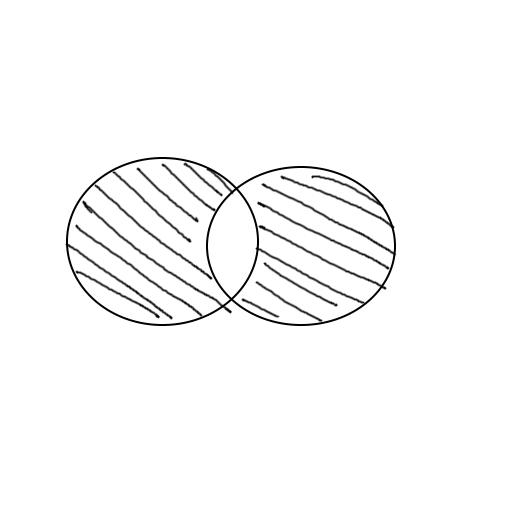
\includegraphics[width=\linewidth]{1.png}
    
    
    \label{fig:1}
\end{figure}

\begin{definition}
    (*)
    Пусть $v_1 \ldots v_n$ и $u_1, u_2, \ldots u_n$ --- базисы

    Выразим базис $u_1 \ldots u_n$ через $v_1 \ldots v_n$:

    $u_1 = a_1 \cdot v_1 + a_2 \cdot v_2 + \ldots + a_n \cdot v_n$
    
    $u_2 = a_2 \cdot v_1 + a_2 \cdot v_2 + \ldots + a_{2n} \cdot v_n$

    $\vdots$

    $u_n = a_n \cdot v_1 + a_{n2} \cdot v_2 + \ldots + a_{nr} \cdot vn$

    Тогда $A = \left(
        \begin{array}{ccc}
            a_{11} & \ldots & a_{1m}\\
            \vdots & \ddots & \vdots\\
            a_{n1} &\ldots & a_{nm}
        \end{array}
        \right)$ -- матрица перехода от $v_1 \ldots v_n$ к $u_1 \ldots u_n$
        

\end{definition}


\begin{definition}
    Пусть есть 
    
    $A = \left(
    \begin{array}{cccc}
        a_{11} & a_{12} & \ldots & a_{1k}\\
        a_{21} & a_{22} & \ldots & a_{2k}\\
        \vdots & \vdots & \ddots & \vdots\\
        a_{n1} &\ldots & \ldots & a_{nk}
    \end{array}
    \right)$ --- Матрица $n \times K$

    
    $B = \left(
    \begin{array}{cccc}
        b_{11} & b_{12} & \ldots & b_{1l}\\
        b_{21} & b_{22} & \ldots & b_{2l}\\
        \vdots & \vdots & \ddots & \vdots\\
        b_{n1} &\ldots & \ldots & b_{nl}
    \end{array}
    \right)$ --- Матрица $k \times l$

    $\space$
    Умножение матриц определяется как:
    
    $A \cdot B := \left(
        \begin{array}{cccc}
            c_{11} & c_{12} & \ldots & c_{1l}\\
            c_{21} & c_{22} & \ldots & c_{2l}\\
            \vdots & \vdots & \ddots & \vdots\\
            c_{k1} &\ldots & \ldots & c_{kl}
        \end{array}
        \right)$

    Элементы матрицы равны:

    $c_{11} = a_{11} \cdot b_{11} + a_{12} \cdot b_{21} + \ldots + a_{1k} \cdot b_{kl}$

    $c_{12} = a_{11} \cdot b_{12} + a_{12} \cdot b_{22} + \ldots + a_{1k} \cdot b_{k2}$
    
    $\vdots$

    $c_{ij} = a_{i1} \cdot b_{1j} + a_{i2} \cdot b_{2j} + \ldots + a_{ik} \cdot b_{kj}$

    $\vdots$

\end{definition}

\begin{remark}
    Выражение базиса через базис можно записать так:

    $\left(
    \begin{array}{c}
        u_{1} \\
        u_{2} \\
        \vdots \\
        u_{n} 
    \end{array}
    \right) \left(
        \begin{array}{ccc}
            a_{11} & \ldots & a_{1n}\\
            a_{21} & \ldots & a_{2n}\\
            \vdots & \ddots & \vdots\\
            a_{n1} &\ldots & a_{nn}
        \end{array}
        \right) \left(
            \begin{array}{c}
                u_{1}\\
                u_{2}\\
                \vdots\\
                u_{n}
            \end{array}
            \right)$    
\end{remark}

\begin{theorem}
    Пусть $v_1 \ldots v_n$ и $u_1, u_2, \ldots u_n$ --- базисы.

    A --- матрица перехода от $v_1 \ldots v_n$ к $u_1 \ldots u_n$
    
    B --- матрица перехода от $w_1 \ldots w_n$ к $v_1 \ldots v_n$

    Тогда матрица перехода от $w_1 \ldots w_n$ к $u_1 \ldots u_n$ равна $A \times B$
\end{theorem}

\begin{proof} Выразим базис $v_1 \ldots v_n$ через $w_1 \ldots w_n$:
    
    $v_1 = b_{11}w_1 + \ldots + b_{1n}w_n$
    
    $\vdots$

    $v_1 = b_{n1}w_1 + \ldots + b_{nn}w_n$
   
    Выразим базис $u_1 \ldots u_n$ через $v_1 \ldots v_n$:

    $u_1 = a_{11}(b_{11}w_1 + \ldots + b_{1n}w_n) + \ldots + a_{1n}(b_{n1}w_1 + \ldots + b_{nn}w_n) = w_1(a_{11}b_{11} + a_{12}b_{21} + \ldots + a_{1n}b_{n1}) + \ldots + w_1(a_{n1}b_{1n} + a_{n2}b_{2n} + \ldots + a_{nn}b_{nn})$

    Мы видим, что базис $u_1 \ldots u_n$ выражается через $w_1 \ldots w_n$, а матрица перехода --- $A \times B$.
\end{proof}

\begin{theorem}
    
    A(BC) = (AB)C 

    Умножение матриц не коммутативно, но ассоциативно.

\end{theorem}


$E = \left(
        \begin{array}{cccc}
            1 & 0 & \ldots & 0\\
            0 & 1 & \ldots & 0\\
            \vdots & \ddots & . &\vdots\\
            0 & 0 & \ldots & 1
        \end{array}
        \right)$ - единичная матрица



        
\begin{remark}
    $u_1 \ldots u_n$, $v_1 \ldots v_n$ --- базисы, выражаются как:
    
    
    $\left(
        \begin{array}{c}
            u_1\\
            \vdots\\
            u_n
        \end{array}
        \right) = A \left(
            \begin{array}{c}
                v_1\\
                \vdots\\
                v_n
            \end{array}
            \right)$


$\left(
    \begin{array}{c}
        v_1\\
        \vdots\\
        v_n
    \end{array}
    \right) = B \left(
        \begin{array}{c}
            u_1\\
            \vdots\\
            u_n
        \end{array}
        \right)$

$A \times B = E$

$B \times A = E$

(A и B) --- обратные матрицы
\end{remark}



\section{Скалярное произведение}

\begin{definition}
    V - векторное пространство

    ($\cdot, \cdot$) : $V \times V \to \R$

    \begin{enumerate}
        \item (u, u) $\geq 0$
        (u, u) = 0 $\Leftrightarrow$ U = 0

        \item $(u_1 + u_2; v) = (u_1, v_1) + (u_2, v)$
        $(u, v_1 + v_2) = (u_, v_1) + (u_1 v_2)$

        \item $\alpha(u, v) = (\alpha u, v) = (u, \alpha v)$
        \item (u, v) = (v, u)
    \end{enumerate}

    V - евклидово пространство
    $(\cdot, \cdot)$ - скалярное произведение
\end{definition}

\begin{eg}
    \begin{enumerate}
        \item $ V = \R^n $
        
        $(a_1, a_2, \ldots, a_n) + (b_1, b_2, \ldots, b_n) := a_1 b_1 + a_2 b_2 + \ldots + a_n b_n$

        
    $\left(
    \begin{array}{ccc}
        a_1 & \ldots & a_n
    \end{array}\right) \left(
                \begin{array}{c}
                    a_1\\
                    \vdots\\
                    a_n
                \end{array}
                \right)$

        \item V - пространство функций (\ldots) 
        $(f(x), g(x)) := \int_a^b f(x)g(x)dx$
    \end{enumerate}
\end{eg}

\begin{definition}
    Пусть V - евклидово пространство, $v \in V$
    
    $|v| := \sqrt{ (v, v) }$

    $cos\angle(u, v) := \frac{(u, w)}{|u| \cdot |v|}$



\end{definition}

\begin{theorem}(Неравенство Коши-Буняковского-Шварца (КБШ))

    $|(u, w)| \leq |u| \cdot |v|$

\end{theorem}

\begin{proof}
    \begin{gather*}
        (u + t v, u+t v) \ge 0 \quad \forall t\\
        (u, u) + (u,t v)+(t v, u) + (t v, t v) \ge 0\\
        |u|^2 + 2t(u,v) + t^2 |v|^2 \ge 0 \quad \forall t\\
        \frac{D}{4} \le 0 \quad (u,v)^2 - |u|^2 |v|^2 \le 0\\
        |(u,v)| \le |u| |v|
    \end{gather*}
\end{proof}

\begin{corollary} (Следствие из КБШ)
    \begin{enumerate}
        
        \item $|a_1 b_1 + a_2 b_2 + \ldots + a_n b_n| \leq \sqrt{a_1^2 + a_2^2 + \ldots + a_n^2} \sqrt{b_1^2 + b_2^2 + \ldots + b_n^2}$
        
        \item $(\int_a^b f(x)g(x)dx)^2 \leq (\int_a^b g(x)dx) \cdot (\int_a^b f(x)dx)$
    \end{enumerate}
\end{corollary}


\begin{definition}
    $u \perp v$, если $(u, b) = 0$
\end{definition}

\begin{definition}
    $v_1 \ldots v_n$ --- ортогональная система, если: 

    $\forall v_i, v_j: v_i \perp v_j, (i \neq j)$    
\end{definition}


 \begin{theorem}
    $v_1 \ldots v_n$ - ортогональная система и в ней нет нулевых векторов $\implies v_1 \ldots v_n$ линейно не зависимы.
 \end{theorem}

 \begin{proof}
    \begin{gather*}
        \alpha_1 v_1 + \ldots + \alpha_n v_n = 0 \\
        \alpha_1 (v_1 v_i) + \alpha_2 (v_2, v_i) + \ldots + \alpha_i (v_i, v_i) + \ldots = 0 \\
        a_i |v_i|^2 = 0\\
        \alpha_i = 0
    \end{gather*}
 \end{proof}

 \begin{definition}
    $u$ --- нормированый или единичный если $|u| = 1$

    $v_1 \ldots v_n$ --- ортонормированные системы, если $v_i \perp v_j$ и $|v_i| = 1$

    $v_1 .. v_i$ --- ОНБ ортонормированный базис
 \end{definition}